

\section{Real World Experiments}

\subsection{Experiment Setup}

\textbf{Real robot benchmark.} \ours is evaluated across 4 tasks on 2 different robots, including an Allegro hand and a gripper. We use one RealSense L515 camera to obtain real-world visual observations. All the tasks are visualized in Figure~\ref{fig:real robot task visualization} and summarized in Table~\ref{table:task summary}. \revise{Our real-world setup and everyday objects used in our tasks are shown in Figure~\ref{fig:real world setup}.} We now briefly describe our tasks:

\begin{figure}[t]
    \centering
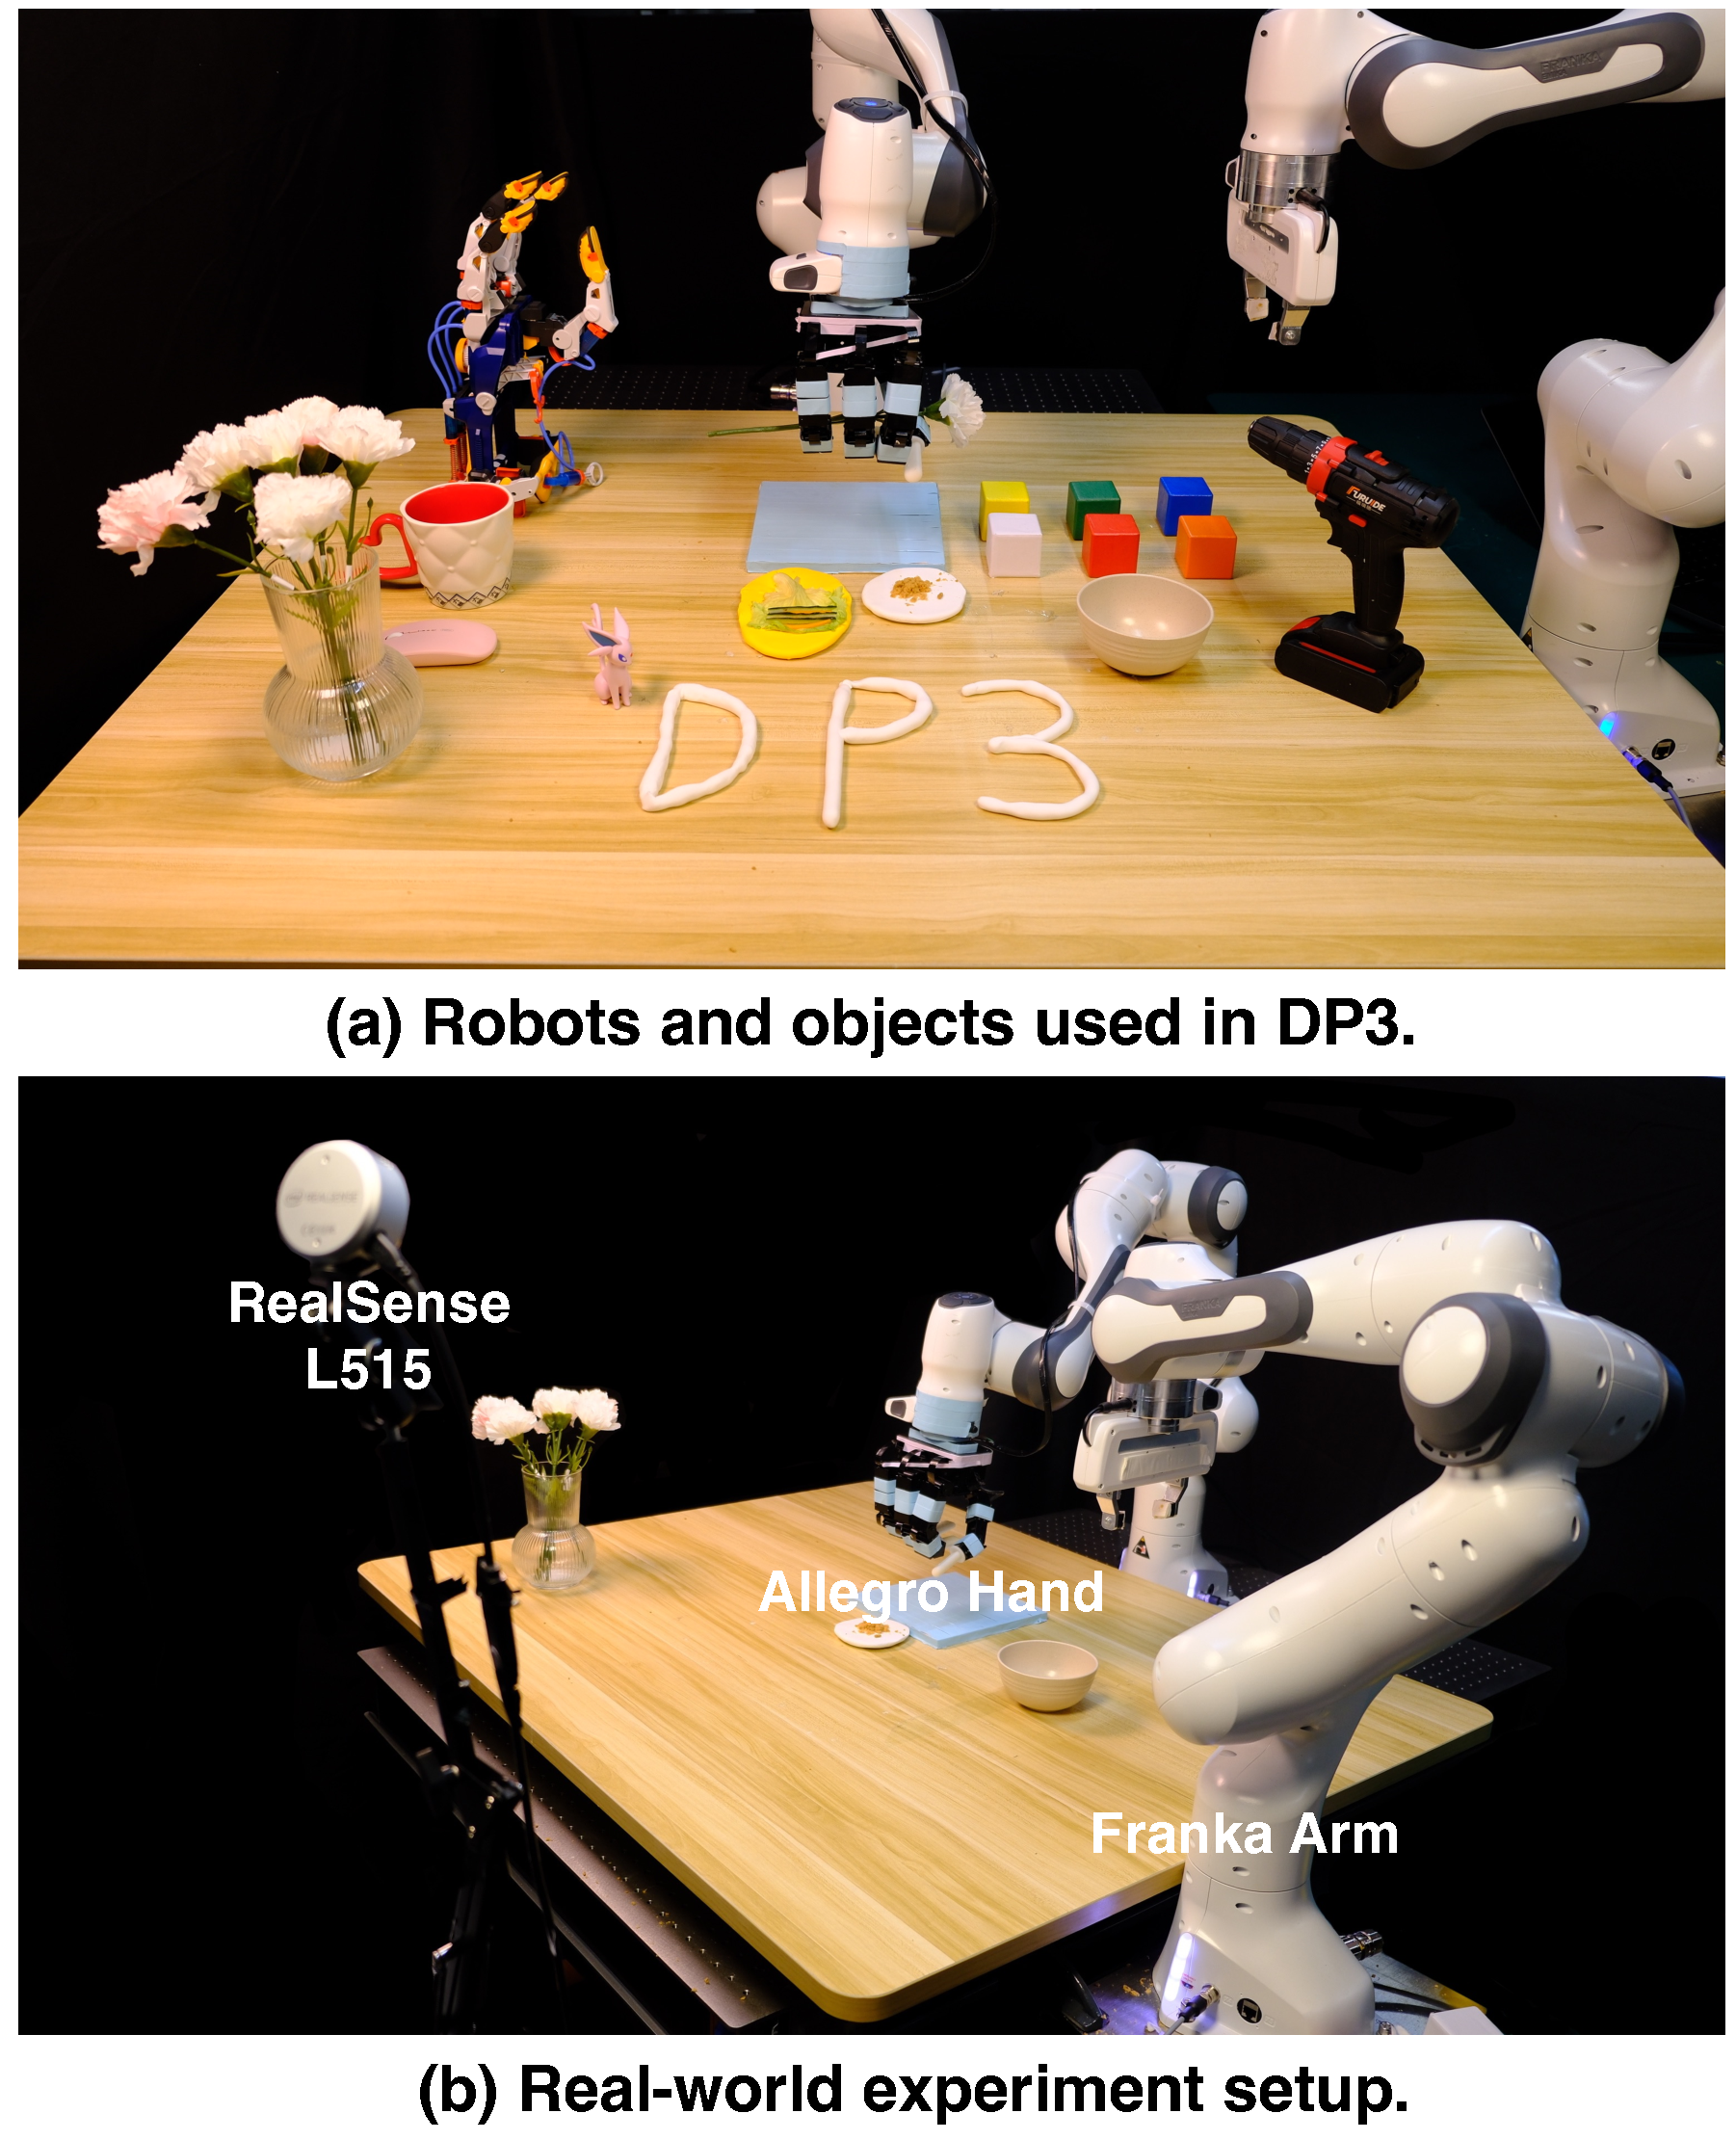
\includegraphics[width=0.49\textwidth]{figures/setup_figure2.pdf}
\vspace{-0.25in}
    \caption{\revise{\textbf{(a) Our robots and objects. (b) Our real-world experiment setup.} We use an Allegro hand and a gripper based on Franka arms and include diverse everyday objects in our manipulation tasks. A RealSense L515 camera is applied to capture visual observations.}}
    \label{fig:real world setup}
    \vspace{-0.25in}
\end{figure}

\begin{enumerate}
    \item \textbf{Roll-Up.} The Allegro hand wraps the plasticine multiple times to make a roll-up. 
    \item \textbf{Dumpling.} The Allegro hand first wraps the plasticine and then pinchs it to make dumpling pleats. 
    \item \textbf{Drill.} The Allegro hand grasps the drill up and moves towards the green cube to touch the cube with the drill.
\item \textbf{Pour.} The gripper grasps the bowl, moves towards the plasticine, pours out the dried meat floss in the bowl, and places the bowl on the table.

\end{enumerate}
\revise{The randomization in each task is shown in Figure~\ref{fig:real task randomness}. For Roll-Up and Dumpling, the plasticine's shape and the appearance of the objects placed upon the plasticine are randomized. For Drill and Pour, the variations come from the random positions of the cube, drill, and bowl.}

Notably, our tasks using the multi-finger hand are carefully designed to show its advantage over the parallel gripper: In Roll-Up and Dumpling, robots could wrap plasticine without requiring extra tools, unlike RoboCook~\citep{shi2023robocook}; In Drill, the drill in the real world is large and heavy, which is quite difficult for the gripper to grasp.



\textbf{Expert demonstrations} are collected by human teleoperation. The Franka arm and the gripper are teleoperated by the keyboard. The Allegro hand is teleoperated with human hands by vision-based retargeting~\citep{qin2023anyteleop,handa2020dexpilot}. Since our tasks contain more than one stage and include complex multi-finger robots and deformable objects, making the process of demonstration collection very time-consuming, we only provide 40 demonstrations for each task.

\textbf{Baselines.} Based on our simulation experiments, image-based and depth-based diffusion policies are still powerful, thus we select them as baselines for real-world experiments. Different vision modalities are visualized in Figure~\ref{fig:different 3d representations}.


\begin{figure}[htbp]
    \centering
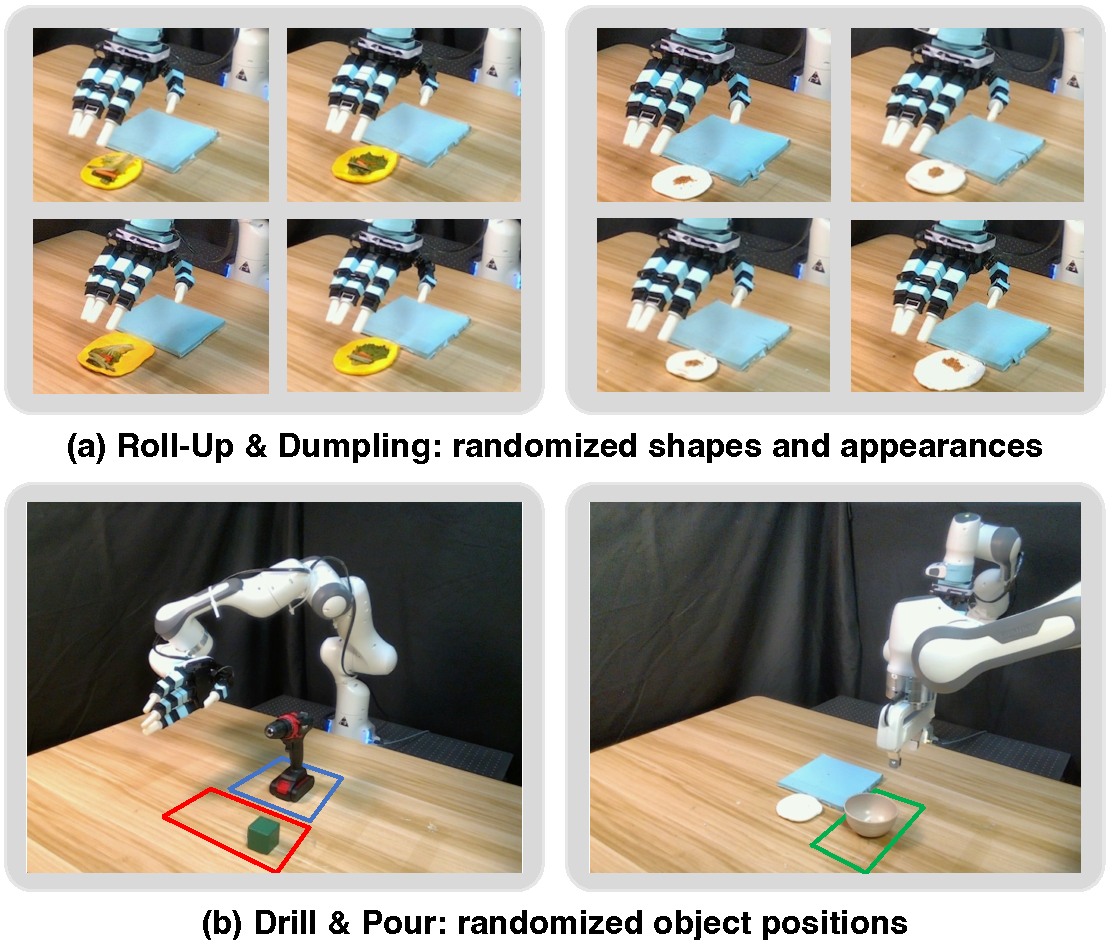
\includegraphics[width=0.5\textwidth]{figures/task_randomness2.pdf}
\vspace{-0.1in}
    \caption{\revise{\textbf{Randomization in collected demonstrations for real-world tasks.} \textbf{Roll-Up}: The shape of the plasticine and the vegetables on it varies in each trajectory. \textbf{Dumpling}: The shape of the plasticine and the distribution of the meat floss on it are different in each trajectory. \textbf{Drill}: The red and blue rectangles respectively mark the range of positions where the cube and drill can be placed. \textbf{Pour}: The green rectangle marks the range of positions of the bowl.}}
    \label{fig:real task randomness}
    \vspace{-0.25in}
\end{figure}


\begin{figure*}[t]
    \centering
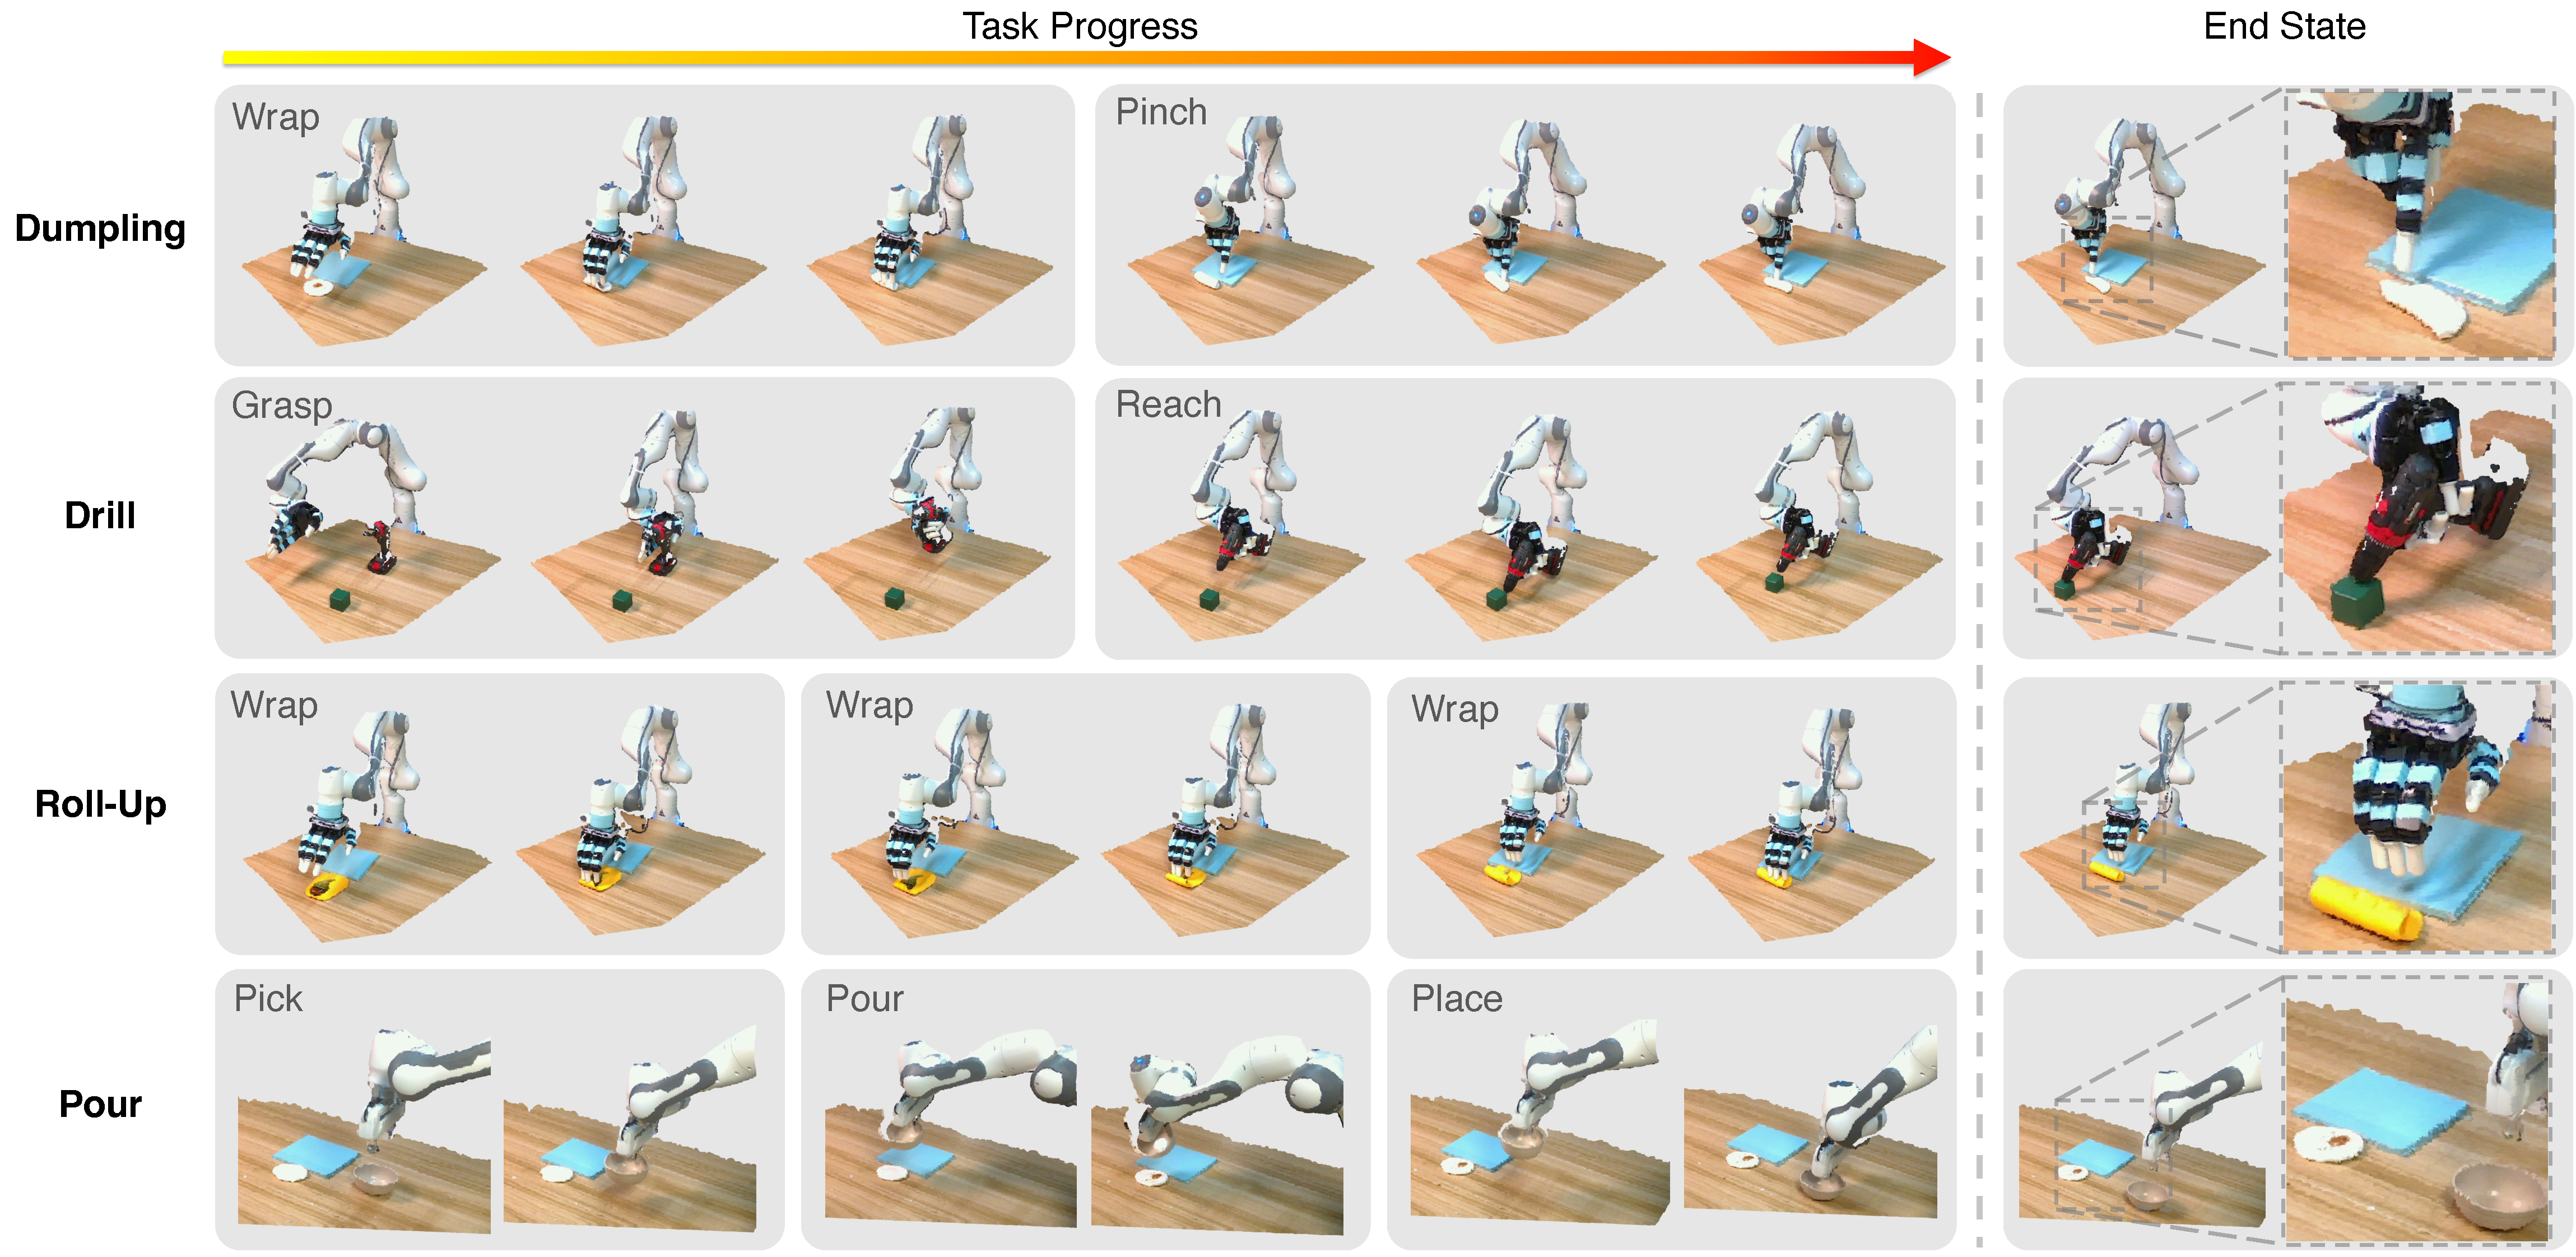
\includegraphics[width=0.99\textwidth]{figures/real_task_visualization.pdf}
\vspace{-0.08in}
    \caption{\textbf{Our real robot benchmark} consists of 4 challenging tasks. The Allegro hand is required to make a \textbf{\textit{Dumpling}}, \textbf{\textit{Drill}} the cube, and make a \textbf{\textit{Roll-Up}}. The gripper is required to \textbf{\textit{Pour}} dried meat floss in the bowl. Each task contains multiple stages. We visualize the point clouds of the collected trajectories.}
    \label{fig:real robot task visualization}
    \vspace{-0.17in}
\end{figure*}






\begin{figure}[t]
    \centering
    % \vspace{-0.05in}
    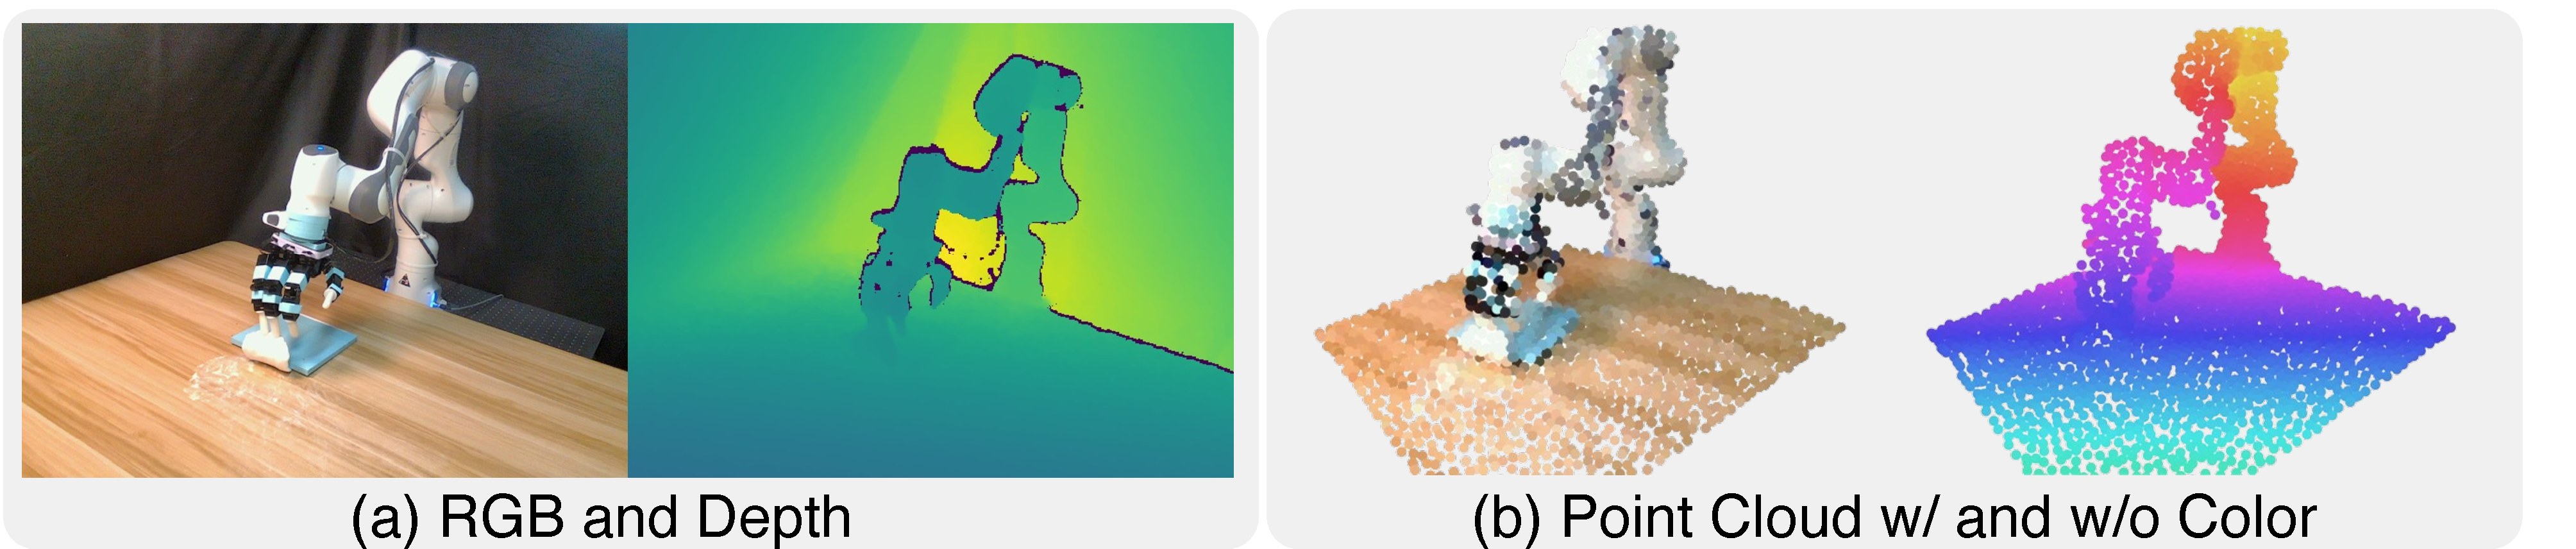
\includegraphics[width=0.5\textwidth]{figures/different_3d_repr.pdf}
    \vspace{-0.22in}
    \caption{\textbf{Different vision modalities in the real world,} include images, depths, and point clouds. }
    \label{fig:different 3d representations}
    \vspace{-0.12in}
\end{figure}


\subsection{Effectiveness}
Results for our real robot tasks are given in Table~\ref{table: main real robot}. Consistent with our simulation findings, we observe in real-world experiments that \ours could handle all tasks with high success rates, given only \textit{40} demonstrations. Interestingly, we also observe that while both image-based and depth-based diffusion policies have comparatively low average accuracies, they exhibit distinct strengths in specific tasks. For instance, the image-based diffusion policy excels in the Drill task but fails entirely in Roll-Up. In contrast, the depth-based policy achieves a notable success rate of $40\%$ in Roll-Up.


\begin{table}[htbp]
\centering
\vspace{-0.1in}
\caption{\textbf{Main results for real robot experiments.} Each task is evaluated with 10 trials.}
\label{table: main real robot}
\vspace{-0.05in}
\resizebox{0.49\textwidth}{!}{%
\begin{tabular}{l|cccc|ccccc}
\toprule


  Real Robot & Roll-Up & Dumpling  & Drill & Pour & \textbf{Average} \\
  

\midrule


Diffusion Policy & \cc{0} & \cc{30} & \cc{70} & \cc{40} & \dd{35.0}{25.0} \\
Diffusion Policy (Depth) & \cc{40} & \cc{20}  &\cc{10} & \cc{10} & \dd{20.0}{12.2} \\
\textbf{\ours} & \ccbf{90} & \ccbf{70} & \ccbf{80} & \ccbf{100} &  \ddbf{85.0}{11.2}\\


\bottomrule
\end{tabular}}
\vspace{-0.2in}
\end{table}




\subsection{Generalization}
Besides the effectiveness in handling all tasks, \ours show strong generalization abilities in the real world. We categorize the generalization abilities of \ours into 4 aspects and detail each aspect as follows.

\textbf{Spatial generalization.} As illustrated in our motivating example, \ours could better extrapolate in 3D space. We demonstrate this property in the real world, as shown in Table~\ref{table: spatial generalization}. We find that baselines fail to generalize to all test positions while \ours succeed in 4 out of 5 trials.

\begin{table}[htbp]
\centering
\vspace{-0.1in}
\caption{\textbf{Spatial generalization on Pour.} We place the bowl at 5 different positions that are unseen in the training data. Each position is evaluated with one trial.}
\label{table: spatial generalization}
\vspace{-0.05in}
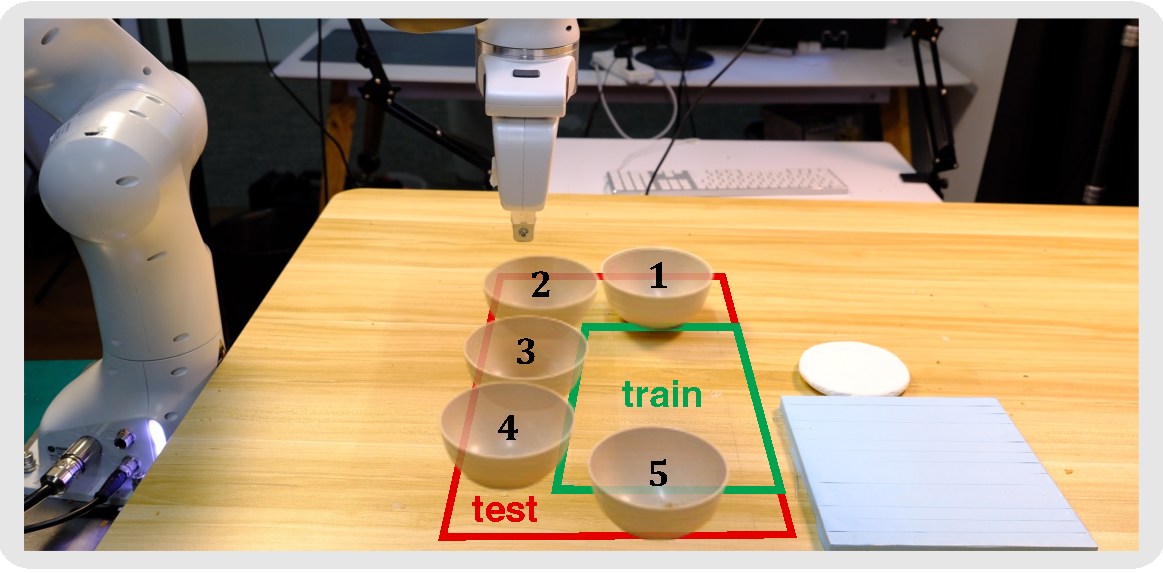
\includegraphics[width=0.40\textwidth]{figures/spatial_generalization.pdf}
\resizebox{0.4\textwidth}{!}{%
\vspace{0.2in}
\begin{tabular}{l|cccccc|ccc}
\toprule


  Spatial Generalization &  1 & 2 & 3 & 4 & 5\\

\midrule
Diffusion Policy & \textcolor{gred}{\XSolidBrush} & \textcolor{gred}{\XSolidBrush} & \textcolor{gred}{\XSolidBrush} & \textcolor{gred}{\XSolidBrush} & \textcolor{gred}{\XSolidBrush} \\
  Diffusion Policy (Depth) & \textcolor{gred}{\XSolidBrush} & \textcolor{gred}{\XSolidBrush} & \textcolor{gred}{\XSolidBrush} & \textcolor{gred}{\XSolidBrush} & \textcolor{gred}{\XSolidBrush} \\
  \textbf{\ours}  & \textcolor{gred}{\XSolidBrush} & \textcolor{ggreen}{\Checkmark} & \textcolor{ggreen}{\Checkmark} & \textcolor{ggreen}{\Checkmark} & \textcolor{ggreen}{\Checkmark} \\
\bottomrule
\end{tabular}}
\vspace{-0.1in}
\end{table}



\textbf{Appearance generalization.} \ours is designed to process point clouds without color information, inherently enabling it to generalize across various appearances effectively. As demonstrated in Table~\ref{table: appearance gen}, \ours consistently exhibits successful generalization to cubes of differing colors, while baseline methods could not achieve. It is noteworthy that the depth-based diffusion policy also does not incorporate color as input. However, due to its lower accuracy on the training object, the ability to generalize is also limited.

One solution to improve the appearance generalization ability of image-based methods is applying strong data augmentation during training~\citep{hansen2022lfs,hansen2021svea}, which however could impede the learning process \citep{yuan2022pieg,hansen2021svea}. More importantly, the primary objective of this work is to demonstrate that \ours, even without the aid of any data augmentation, can effectively generalize, thereby underscoring the potential of 3D representations in real robot learning.

\begin{table}[htbp]
\centering
\vspace{-0.05in}
\caption{\textbf{Appearance generalization on Drill.} Algorithms are trained with the green cube only and evaluated on 5 different colored cubes. Each color is evaluated with one trial.}
\label{table: appearance gen}
\vspace{-0.05in}
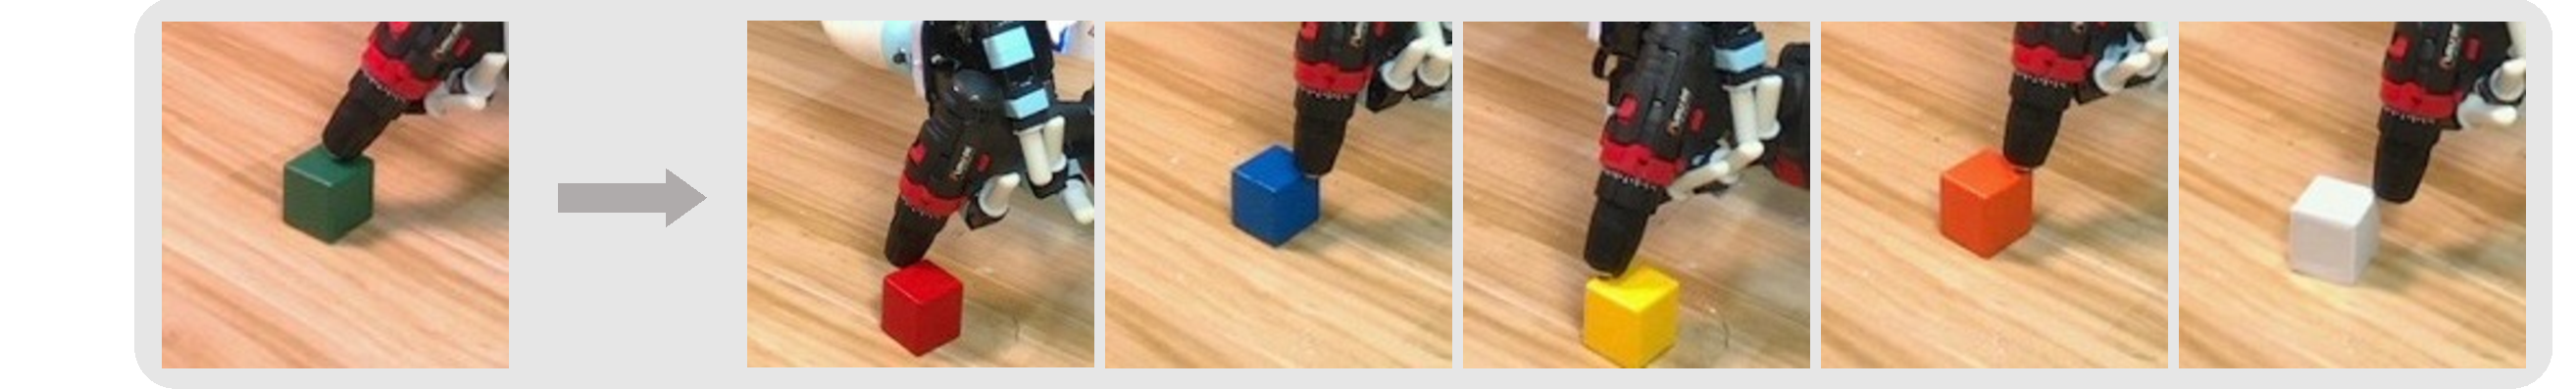
\includegraphics[width=0.48\textwidth]{figures/gen_appear.pdf}
\resizebox{0.4\textwidth}{!}{%

\begin{tabular}{l|ccccccccc}
\toprule


Apperance Generalization (\textcolor{ggreen}{$\blacksquare$}) & \textcolor{red}{$\blacksquare$}  & \textcolor{blue}{$\blacksquare$}  & \textcolor{yellow}{$\blacksquare$}    & \textcolor{orange}{$\blacksquare$}  & \textcolor{grey}{$\blacksquare$}  \\
% \midrule
% 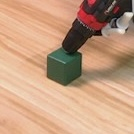
\includegraphics[width=0.15\linewidth]{figures/appear_gen/green.jpg}&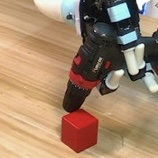
\includegraphics[width=0.15\linewidth]{figures/appear_gen/red.jpg}&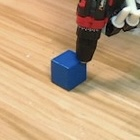
\includegraphics[width=0.15\linewidth]{figures/appear_gen/blue.jpg}&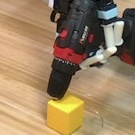
\includegraphics[width=0.15\linewidth]{figures/appear_gen/yellow.jpg}&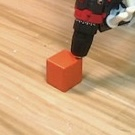
\includegraphics[width=0.15\linewidth]{figures/appear_gen/orange.jpg}&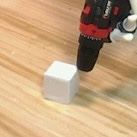
\includegraphics[width=0.15\linewidth]{figures/appear_gen/white.jpg}\\

\midrule
  Diffusion Policy & \textcolor{gred}{\XSolidBrush} & \textcolor{gred}{\XSolidBrush} & \textcolor{gred}{\XSolidBrush} & \textcolor{gred}{\XSolidBrush} & \textcolor{gred}{\XSolidBrush} \\
  Diffusion Policy (Depth) & \textcolor{gred}{\XSolidBrush} & \textcolor{gred}{\XSolidBrush} & \textcolor{gred}{\XSolidBrush} & \textcolor{gred}{\XSolidBrush} & \textcolor{gred}{\XSolidBrush} \\
  \textbf{\ours}  & \textcolor{ggreen}{\Checkmark} & \textcolor{ggreen}{\Checkmark} & \textcolor{ggreen}{\Checkmark} & \textcolor{ggreen}{\Checkmark} & \textcolor{ggreen}{\Checkmark} \\
\bottomrule
\end{tabular}}
\vspace{-0.1in}
\end{table}




\textbf{Instance generalization.} Achieving generalization across diverse instances, which vary in shape, size, and appearance, presents a significantly greater challenge compared to mere appearance generalization. In Table~\ref{table: instance gen}, we demonstrate that \ours effectively manages a wide range of everyday objects. This success can be primarily attributed to the inherent characteristics of point clouds. Specifically, the use of point clouds allows for policies that are less prone to confusion, particularly when these point clouds are downsampled. This feature significantly enhances the model's ability to adapt to varied instances.

\begin{table}[htbp]
\centering
\vspace{-0.05in}
\caption{\textbf{Instance generalization on Drill.} We replace the cube used in Drill with five objects in varied sizes from our daily life. Each instance is evaluated with one trial.}
\vspace{-0.05in}
\label{table: instance gen}
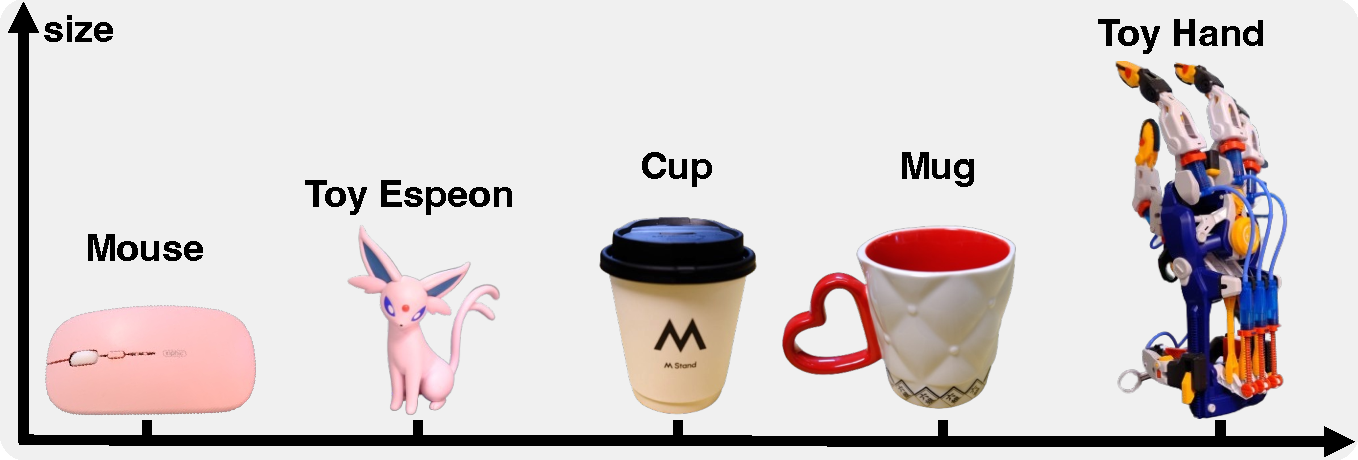
\includegraphics[width=0.49\textwidth]{figures/instance.pdf}
\resizebox{0.49\textwidth}{!}{%

\begin{tabular}{l|ccccccccc}
\toprule


Instance Generalization & Mouse & Espeon   & Cup    & Mug & Hand  \\

% 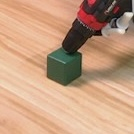
\includegraphics[width=0.15\linewidth]{figures/appear_gen/green.jpg}&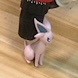
\includegraphics[width=0.15\linewidth]{figures/instance_gen/cat.jpg}&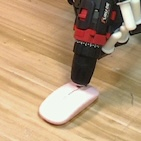
\includegraphics[width=0.15\linewidth]{figures/instance_gen/mouse.jpg}&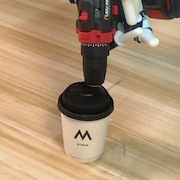
\includegraphics[width=0.15\linewidth]{figures/instance_gen/latte.jpg}&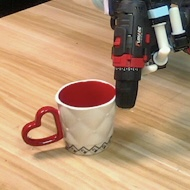
\includegraphics[width=0.15\linewidth]{figures/instance_gen/cup.jpg}&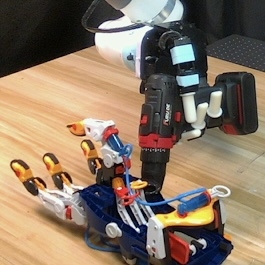
\includegraphics[width=0.15\linewidth]{figures/instance_gen/hand.jpg}\\


\midrule
  Diffusion Policy & \textcolor{gred}{\XSolidBrush} & \textcolor{gred}{\XSolidBrush} & \textcolor{gred}{\XSolidBrush} & \textcolor{gred}{\XSolidBrush} & \textcolor{ggreen}{\Checkmark} \\
  Diffusion Policy (Depth) & \textcolor{gred}{\XSolidBrush} & \textcolor{gred}{\XSolidBrush} & \textcolor{ggreen}{\Checkmark} & \textcolor{gred}{\XSolidBrush} & \textcolor{gred}{\XSolidBrush} \\
  \textbf{\ours}  & \textcolor{ggreen}{\Checkmark} & \textcolor{ggreen}{\Checkmark} & \textcolor{ggreen}{\Checkmark} & \textcolor{ggreen}{\Checkmark} & \textcolor{ggreen}{\Checkmark} \\
\bottomrule
\end{tabular}}
% \vspace{-0.1in}
\end{table}




\textbf{View generalization.} Generalizing image-based methods across different views is notably challenging~\citep{yang2023movie}, and acquiring training data from multiple views can be time-consuming and costly~\citep{ze2023gnfactor,shen2023distilled}. We demonstrate in Table~\ref{table: view gen} that \ours effectively addresses this generalization problem when the camera views are altered slightly. It is important to note that since the camera view is altered, we manually \revise{transform the point clouds} and adjust the cropped space of the point clouds. \revise{Accurate transformation isn't necessary due to the robustness of our network. However, it is crucial to acknowledge that while the network can generalize across minor variations in camera views, significant changes might be hard to handle.}

% This adjustment allows \ours to seamlessly generalize across views.~\gu{Do we need this sentence?}

\begin{table}[htbp]
\vspace{-0.1in}
\centering
\caption{\textbf{View generalization on Roll-Up.} Each view is evaluated with one trial.}
\vspace{-0.05in}
\label{table: view gen}
   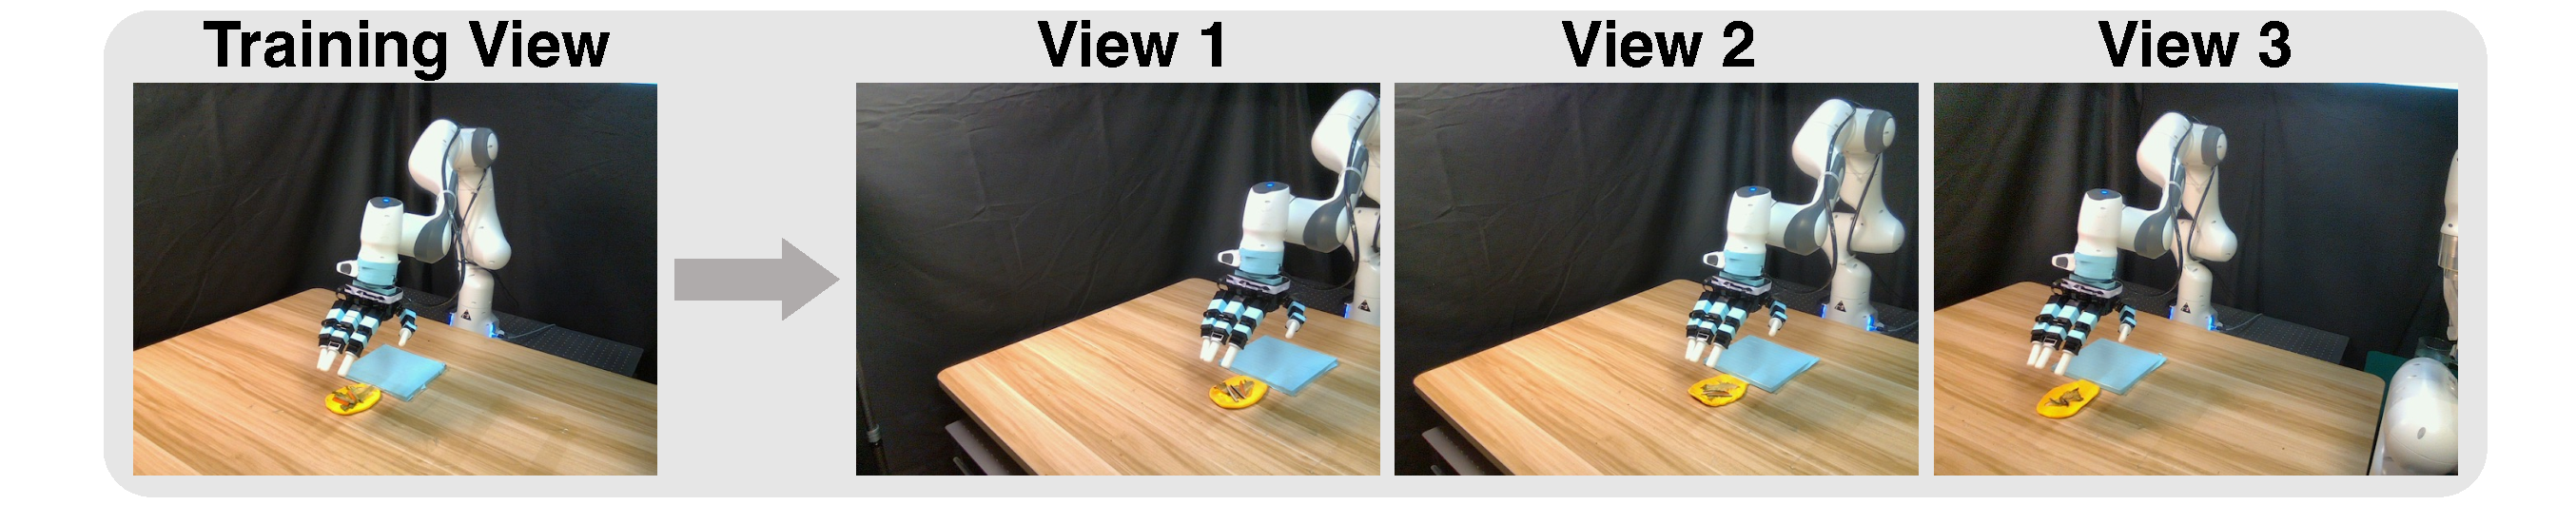
\includegraphics[width=0.48\textwidth]{figures/view_gen.pdf}
\resizebox{0.4\textwidth}{!}{%
\begin{tabular}{l|cccccc|ccc}
\toprule


View Generalization & View 1  & View 2  & View 3   \\


\midrule
  Diffusion Policy & \textcolor{gred}{\XSolidBrush} & \textcolor{gred}{\XSolidBrush} & \textcolor{gred}{\XSolidBrush} \\
  Diffusion Policy (Depth) & \textcolor{gred}{\XSolidBrush} & \textcolor{gred}{\XSolidBrush} & \textcolor{gred}{\XSolidBrush} \\
  \textbf{\ours}  & \textcolor{ggreen}{\Checkmark} & \textcolor{ggreen}{\Checkmark} & \textcolor{ggreen}{\Checkmark}  \\
  
\bottomrule
\end{tabular}}
\vspace{-0.1in}
\end{table}



\revise{
\textbf{Cluttered Scenes}. Despite the simplicity of the DP3 Encoder, we demonstrate that DP3 is capable of handling tasks in complex real-world cluttered environments. To illustrate this, we design a pick \& place task (i.e. pick the cube and place it in the bowl) set in cluttered scenes using a gripper and collect 50 demonstrations for training. The results presented in Table~\ref{table: ablation cluttered scenes} show that DP3 solves the task with a high success rate. Aligning with our simulation experiments, DP3 equipped with PointNeXt fails to address the task. Meanwhile, DP3 using color point clouds as input performs comparably to the original DP3 when picking the training yellow cube, yet it struggles with other colored cubes and diverse objects. This demonstrates the effectiveness and generalization ability of DP3 in complex scenes.
}

\begin{table}[htbp]
\centering
\vspace{-0.1in}
\caption{\revise{\textbf{Results in cluttered scenes.} Each algorithm is evaluated with 10 trials in the training color. Each out-of-domain color and object are evaluated with one trial.}}
\label{table: ablation cluttered scenes}
\vspace{-0.05in}
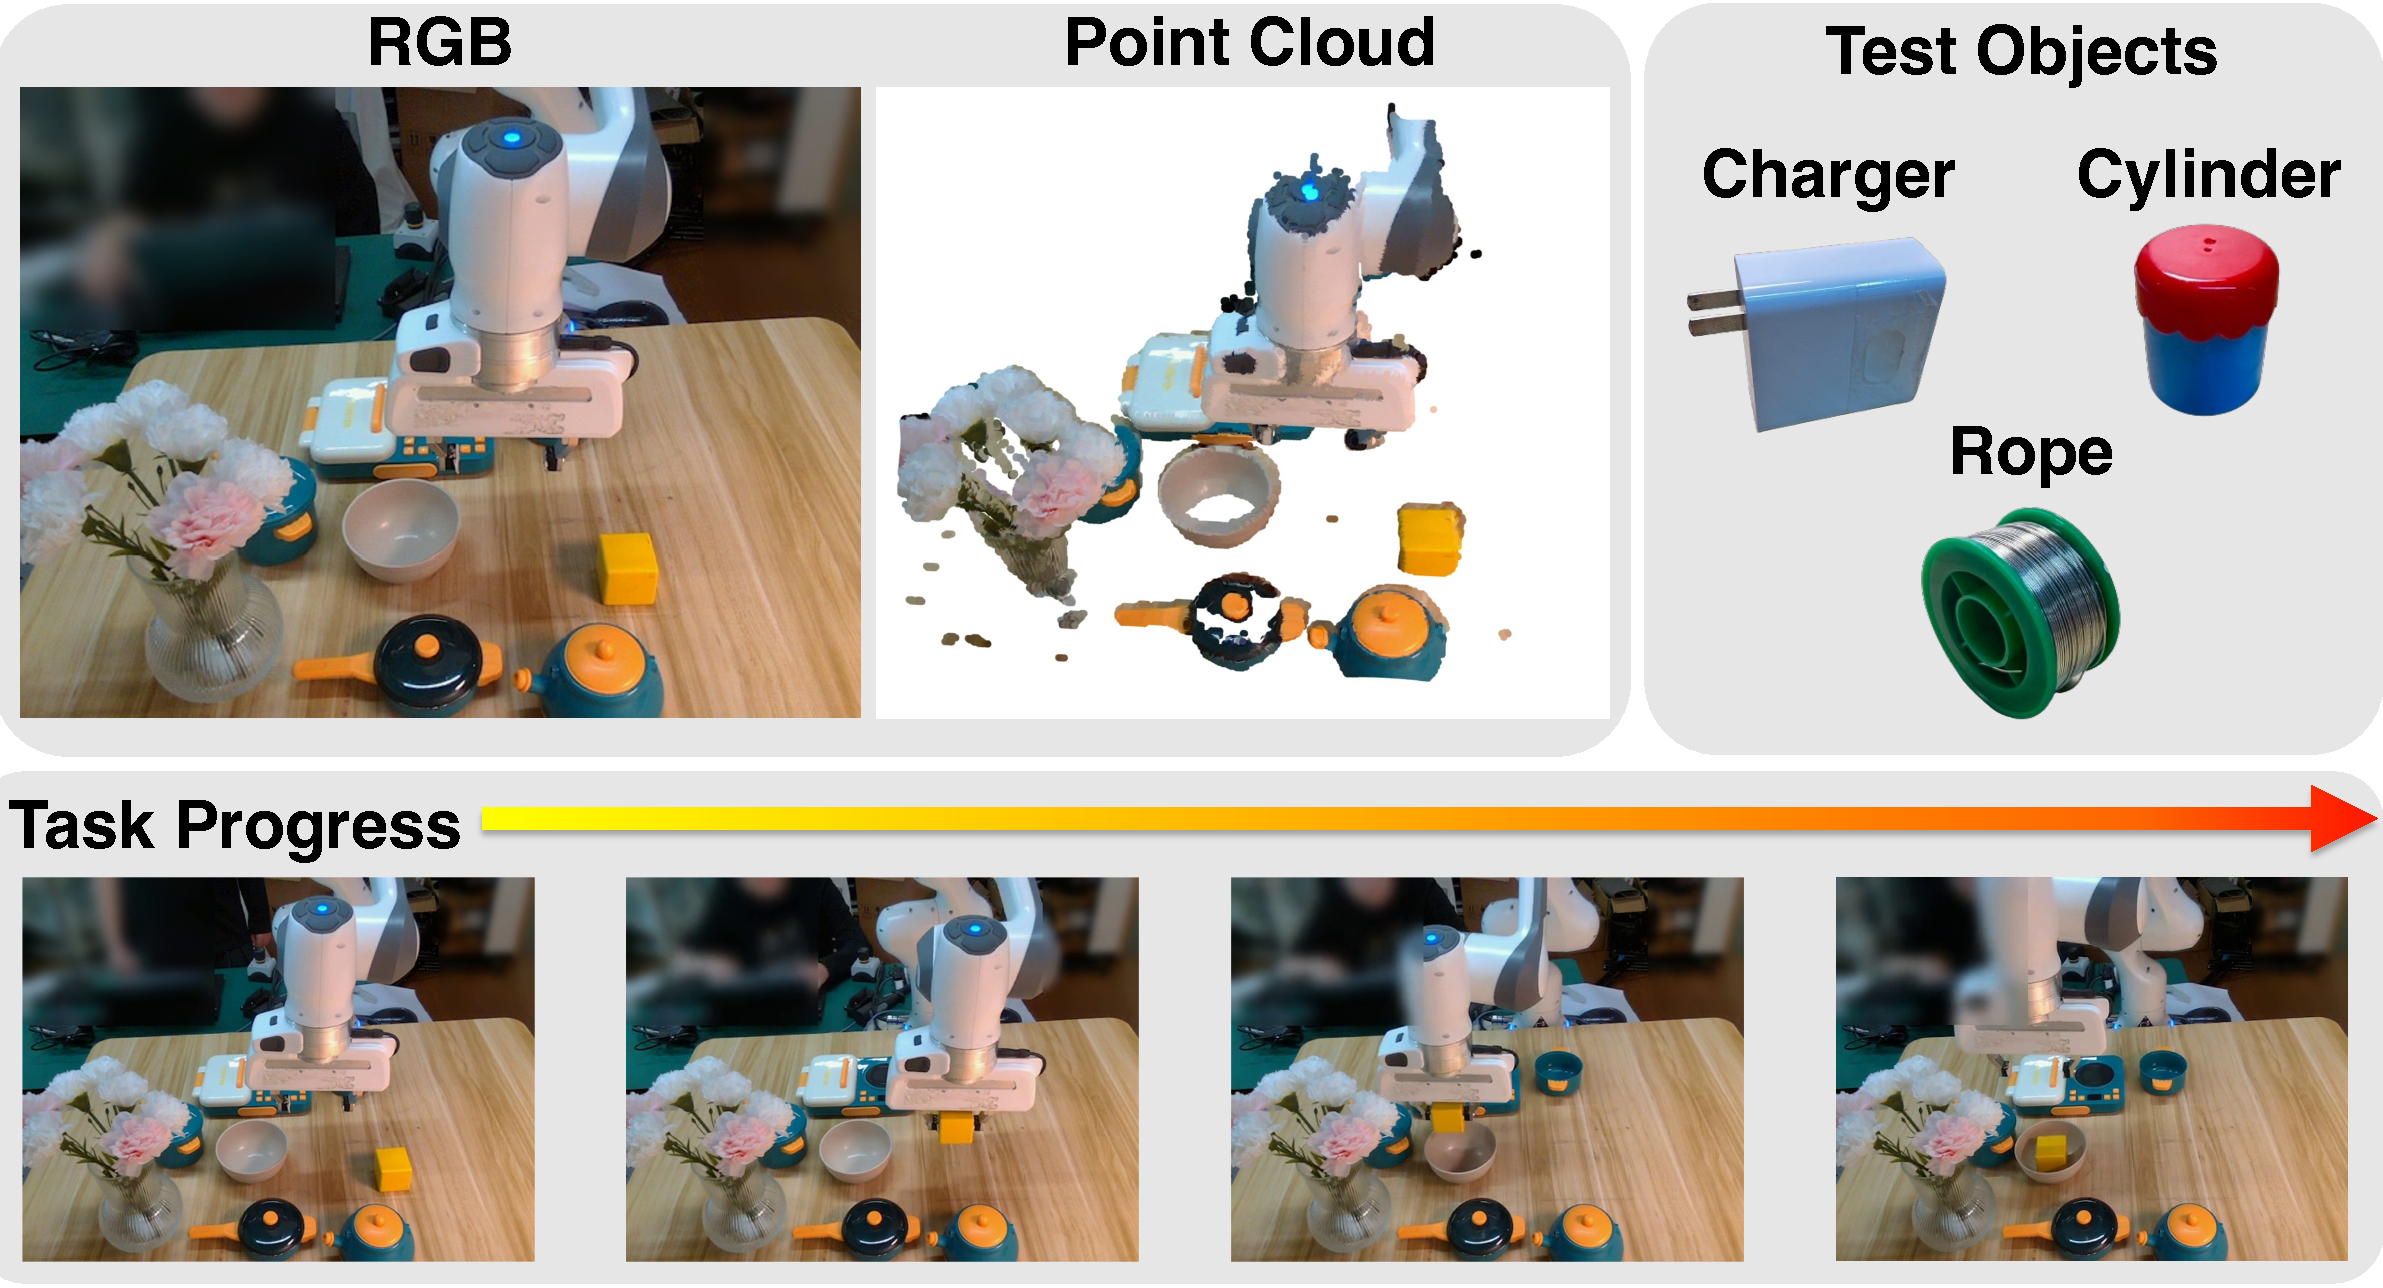
\includegraphics[width=0.48\textwidth]{figures/cluttered.pdf}

\resizebox{0.49\textwidth}{!}{%
\begin{tabular}{l|ccccccccc}
\toprule


  Cluttered Scenes  & Diffusion Policy & DP3 w/ PointNeXt  & DP3 w/ color & DP3 \\
\midrule

  Success Rate &  \cc{60} & \cc{0} & \ccbf{80}   & \ccbf{80}\\



\midrule
\end{tabular}}


\resizebox{0.49\textwidth}{!}{%
\begin{tabular}{l|ccc|cccccc}
\midrule


  Train with \textcolor{yellow}{$\blacksquare$} Cube & \textcolor{red}{$\blacksquare$} & \textcolor{blue}{$\blacksquare$} & \textcolor{ggreen}{$\blacksquare$} & Charger & Cylinder & Rope \\
\midrule
 DP3 w/ color & \textcolor{gred}{\XSolidBrush} &
\textcolor{gred}{\XSolidBrush} &
\textcolor{gred}{\XSolidBrush} &\textcolor{gred}{\XSolidBrush} &
\textcolor{gred}{\XSolidBrush} &
\textcolor{gred}{\XSolidBrush} \\
DP3  &  \textcolor{ggreen}{\Checkmark} & \textcolor{ggreen}{\Checkmark} & \textcolor{ggreen}{\Checkmark} &  \textcolor{ggreen}{\Checkmark} & \textcolor{ggreen}{\Checkmark} & \textcolor{ggreen}{\Checkmark} \\




\bottomrule
\end{tabular}}




\end{table}







\subsection{\revise{Observation on Deployment Safety}}
\label{section: safe deployment}
In our real-world experiments, we observe that image-based and depth-based diffusion policies often deliver unpredictable behaviors in real-world experiments, which necessitates human termination to ensure robot safety. We define this situation as \textit{safety violation} and compute the safety violation rate in our main real-world experiments, shown in Table~\ref{table: safety violation}. Interestingly and surprisingly, we find that \ours rarely violates the safety, showing that \ours is a practical and hardware-friendly method for real robot learning. \revise{An intuitive explanation is that since the robots operate in 3D space, directly observing 3D information helps avoid collision. It is important to note that our assessment of safety is primarily qualitative. We intend to explore a more theoretical understanding of this observation in our future work.}



\begin{table}[htbp]
\centering
% \vspace{-0.1in}
\caption{\textbf{Safety violation rate.} While conducting the main real-world experiments, we also count the times of safety violation and compute the rate.}
\label{table: safety violation}
\vspace{-0.05in}
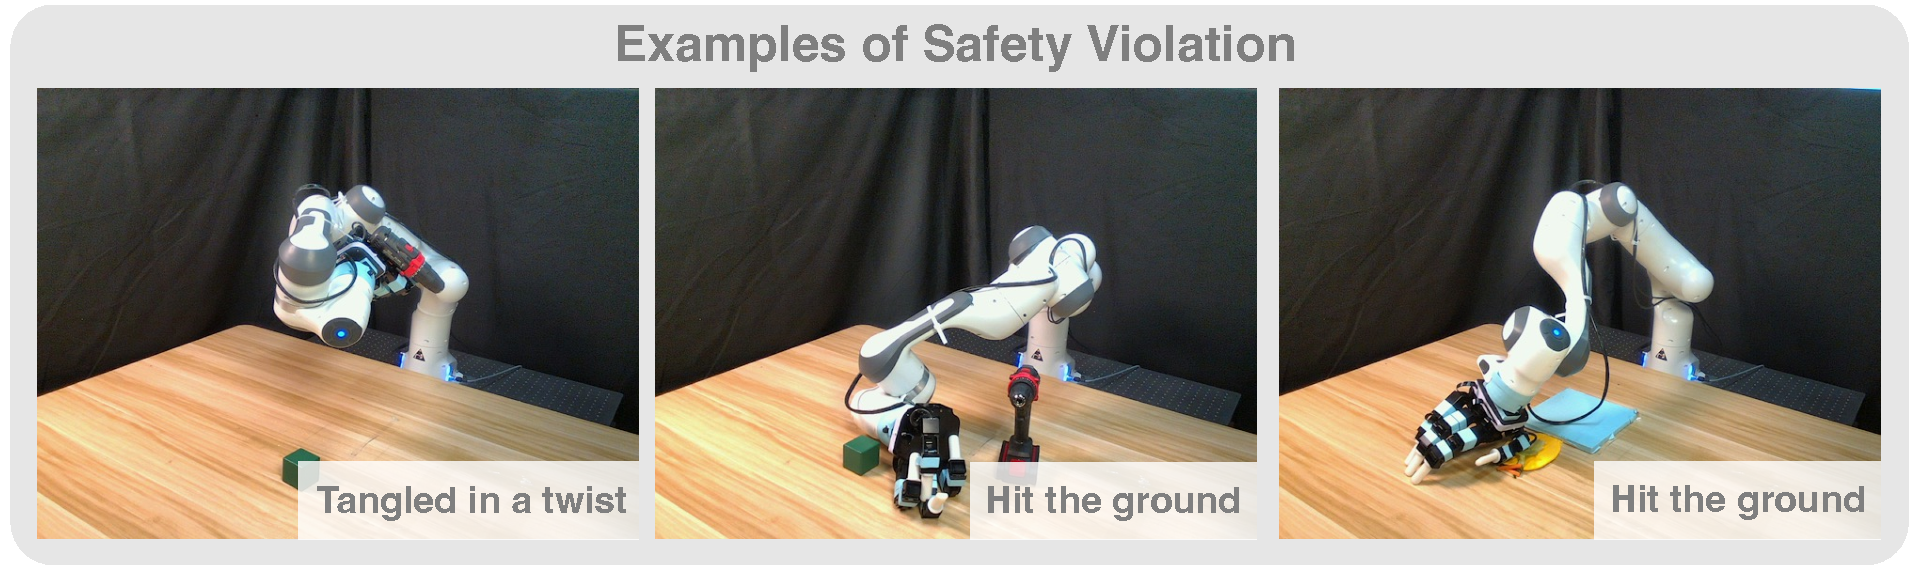
\includegraphics[width=0.5\textwidth]{figures/safety.pdf}

\resizebox{0.49\textwidth}{!}{%
\begin{tabular}{l|cccc|ccccc}
\toprule


  Safety Violation Rate $\downarrow$ & Roll-Up & Dumpling  & Drill & Pour & \textbf{Average} \\

\midrule


Diffusion Policy &\cc{90} & \cc{20} & \cc{20} & \cc{0} & \cc{32.5}\\
Diffusion Policy (Depth) & \cc{20} & \cc{30} & \cc{30} & \cc{20} & \cc{25.0}\\
\textbf{\ours} & \ccbf{0} & \ccbf{0} & \ccbf{0} &\ccbf{0} & \ccbf{0.0}\\

\bottomrule
\end{tabular}}
\vspace{-0.15in}
\end{table}



